\documentclass[12pt]{article}
\usepackage[margin=1in]{geometry}
\usepackage{amsmath}
\usepackage{amssymb}
\usepackage{amsfonts}
\usepackage{amsthm}
\newtheorem{thm}{Theorem}[section]
\newtheorem{cor}[thm]{Corollary}
\newtheorem{lem}[thm]{Lemma}
\newtheorem{prop}[thm]{Proposition}
\usepackage{tikz-cd}
\renewcommand{\d}{\mathrm{d}}

\begin{document}

\title{Math 180 Homework 7}
\author{Nathan Solomon}
\maketitle

\section{}
\noindent\fbox{\fbox{\parbox{6.5in}{
            Prove or disprove: if $T$ is a minimal spanning tree of a weighted graph $(G, \operatorname{wt})$ and $u,v$ are two vertices, then the $u,v$-path in $T$ is a minimal weight $u,v$-path in $G$.
}}}\bigskip\par
False. Consider the cycle graph $C_{100}$, where $u,v$ are two adjacent vertices, the edge between them has weight 2, and every other edge has weight 1. Then the only minimal spanning tree $T$ is the path graph $P_{99}$ in which $u$ and $v$ are leaves, so the path between them in $T$ has weight 99. But in $G$, there is a path between $u$ and $v$ with weight 2, so the path in $T$ (which has weight 99) is not minimal in $G$.
\par
\textit{Note: this was the first example I though of, but a simpler example would be $G=C_3$, where all edges in $G$ have weight 1. For any two distinct vertices $u,v$ in $G$, there is an MST $T$ of $G$ such that $u,v$ are not adjacent in $T$. Then the path between them in $T$ has weight 2, but there is a path between them in $G$ of weight 1.}

\section{}
\noindent\fbox{\fbox{\parbox{6.5in}{
            Let $T$ be a minimal spanning tree in a connected weighted graph $(G, \operatorname{wt})$. Prove that $T$ omits a heaviest edge from every cycle in $G$.
}}}\bigskip\par
Let $e$ be the heaviest edge in some cycle $C$ contained in $G$, and let $e'$ be any other edge in $C$. Then removing $e$ from $T$ and adding in $e'$ will decrease the weight of $T$ by $ \operatorname{wt}(e)- \operatorname{wt}(e') > 0$. Replacing $e$ with $e'$ will not change the fact that all vertices of $G$ are connected in $T$, because the vertices in the cycle are still connected to each other, and every connected component of $G-C$ is still connected in $G$ to at least one of the vertices in $C$. We also will not change the fact that $T$ is a tree, because a connected component is a tree iff $|V|-|E|=1$, and we didn't change either $|V|$ or $|E|$. This new tree is a spanning tree with less weight than the original.
\par
Therefore if $T$ were a minimal tree, it could not contain a heaviest edge from any cycle in $G$.

\section{}
\noindent\fbox{\fbox{\parbox{6.5in}{
    \textbf{Section 5.4, Exercise 4.} Let $G$ be a connected graph with a weight function $w$ on the edges, and assume that $w$ is injective. Prove that the minimum spanning tree of $G$ is determined uniquely.
}}}\bigskip\par
Since there is a unique way to order the edges of $G$ from lowest to highest weight, there is only one possible output of Kruskal's algorithm. Let $T$ be that output, and let $T'$ be a different MST of $G$. Let $e$ be an edge which $T$ contains but $T'$ does not. Then $T'+e$ contains a cycle $C$, and there is some edge $e'$ which is in $C$ but not in $T$. Now $T+e-e'$ is a spanning tree of $G$. Because $T$ has minimal weight of all spanning trees, $w(T+e-e')>w(T)$, which implies $w(e)>w(e')$. But by the exact same logic, $T'+e'-e$ must be a spanning tree, and since $T'$ is an MST, $w(e')>w(e)$. This is a contradiction, so there cannot be any MST of $G$ which is different from $T$.

\section{}
\noindent\fbox{\fbox{\parbox{6.5in}{
    \textbf{Section 8.1, Exercise 3.} \textit{Hint: Count the number of spanning trees along with an edge to remove.}
    \par
    Put $T_n=T(K_n)$. Prove the recurrent formula
    \[ (n-1) T_n = \sum_{k=1}^{n-1} k(n-k) \binom{n-1}{k-1}T_kT_{n-k}. \]
    \textit{Remark.} Theorem 8.1.1 (Cayley's Formula) can be derived from this recurrence too, but it's not so easy.
}}}\bigskip\par
Every spanning tree of $K_n$ vertices can be constructed by the following process:
\begin{enumerate}
    \item Pick some integer $k \in [1,n-1]$.
    \item Split the vertices of $K_n$ into two groups: $G_1$, which contains $k$ vertices, and $G_2$, which contains the other $n-k$ vertices. WLOG, assume $G_1$ contains the vertex labeled 1. There are $\binom{n-1}{k-1}$ ways to make this choice.
    \item Pick a spanning tree for the vertices in $G_1$, and a spanning tree for the vertices in $G_2$. There are $T_kT{n-k}$ ways to make these two choices.
    \item Pick any vertex in $G_1$ and any vertex in $G_2$. There are $k(n-k)$ ways to make this choice. Connect those two vertices by an edge to obtain a spanning tree of $K_n$.
    \end{enumerate}
\par
This construction will always give a spanning tree, but we need to worry now about overcounting. Given a spanning tree of $K_n$, we can choose any of the $n-1$ edges to be the bridge constructed between $G_1$ and $G_2$ in step 4. Then it becomes easy to go through the 4 steps in reverse and identify the choices made at each step. In fact, once we choose which edge in our spanning tree is the bridge between $G_1$ and $G_2$, all the other decisions are uniquely determined. Therefore, the number of spanning trees of $K_n$ with one edge labeled as the bridge is $(n-1)T_n$, but it's also equal to
\[ \sum_{k=1}^{n-1} k (n-k) \binom{n-1}{k-1} T_k T_{n-k}. \]

\section{}
\noindent\fbox{\fbox{\parbox{6.5in}{
            Find the spanning tree of $K_9$ with Prüfer code $(2,8,9,4,7,7,2)$.
}}}\bigskip\par
Using the algorithm from the lecture notes, we make a list of vertices which have not yet been connected to the spanning tree, called $A$, and we repeatedly add an edge to our spanning tree which connects the first element ($a_j$) from the Prüfer code $C$ to the smallest-numbered vertex ($a_i$) which is in $A$ but not in $C$. After each step, we remove $a_j$ from $C$ and $a_i$ from $A$. Once $C$ is empty, we use the last 2 elements of $A$ to make one last edge.
\begin{center}
    \begin{tabular}{|c|c|c|c|}
        \hline
        $C$ & $A$ & $a_j$ & $a_i$ \\
        \hline
        2894772 & 123456789 & 2 & 1 \\
        894772 & 23456789 & 8 & 3 \\
        94772 & 2456789 & 9 & 5 \\
        4772 & 246789 & 4 & 6 \\
        772 & 24789 & 7 & 4 \\
        72 & 2789 & 7 & 8 \\
        2 & 279 & 2 & 7 \\
        & 29 & & \\
        \hline
    \end{tabular}
\end{center}
The list of edges $(a_j, a_i)$ we obtained is
\[ \left\{ (2,1),(8,3),(9,5),(4,6),(7,4),(7,8),(2,7),(2,9) \right\} \]
This gives us the following graph:
\begin{center}
    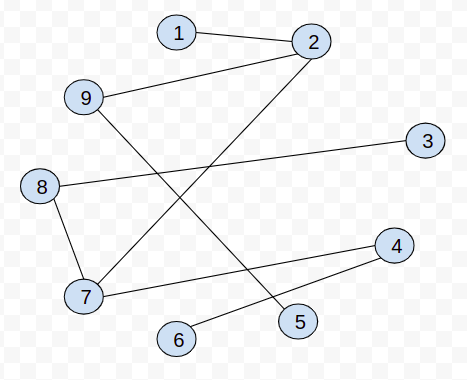
\includegraphics[width=\textwidth]{kruskal_tree.png}
\end{center}
which can also be drawn as
\begin{center}
    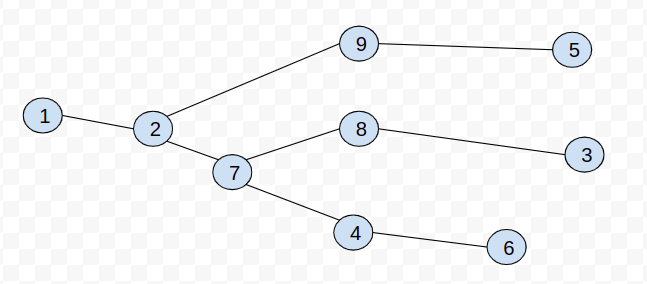
\includegraphics[width=\textwidth]{tree_2.png}
\end{center}


\section{}
\noindent\fbox{\fbox{\parbox{6.5in}{
    Determine the number of spanning trees $T$ of $K_9$ in each of the following scenarios:
    \begin{enumerate}
        \item $T$ has 5 and 8 as leaves.
        \item $T$ does not have 5 as a leaf.
    \end{enumerate}
}}}\bigskip\par
A Prüfer code for a spanning tree $T$ on $n$ vertices is a sequence of $n-2$ numbers from the alphabet $[n]$, and the number of times a number $i \in [n]$ appears in that code is one less than the degree of the vertex labeled $i$ in $T$. Therefore, the vertex labeled $i$ is a leaf of $T$ iff it never appears in the Prüfer code of $T$.
\begin{enumerate}
    \item This is equivalent to counting how many 7-letter words there are from the alphabet $[9]$ which do not contain 5 or 8, but that's equivalent to counting how many 7-letter words there are from the alphabet $[7]$, which is
        \[ 7^7=823543. \]
    \item This is equivalent to counting how many 7-letter words there are from the alphabet $[9]$ which contain 5 at least once. That count is equal to the number of 7-letter words from the alphabet $[9]$, minus the number of 7-letter words from the alphabet $[8]$. That is equal to
        \[ 9^7-8^7=2685817. \]
\end{enumerate}

\section{}
\noindent\fbox{\fbox{\parbox{6.5in}{
    Determine which trees have Prüfer codes that have distinct values in all positions.
}}}\bigskip\par
We know that the number of times a vertex $v$ appears in a Prüfer code is one less than the degree of $v$. The $n-2$ vertices which occur in the Prüfer code exactly once must have degree 2, and the 2 vertices which never appear in the Prüfer code have degree 1. Therefore, if the Prüfer code for a tree $T$ doesn't repeat any numbers, then $T$ is a path graph.

\end{document}
